\subsubsection{Projection of Run-2 ATLAS searches for MSSM heavy Higgs bosons}
%-------------------------------------------------------------------------------
\paragraph{Introduction}
\label{sec:intro}
%-------------------------------------------------------------------------------

The discovery of the Standard Model (SM) like Higgs boson ~\cite{ATLASHiggsJuly2012, CMSHiggsJuly2012}
at the Large Hadron Collider (LHC)~\cite{LHC} has provided important insight into the mechanism of 
electroweak symmetry breaking. However, it remains possible that the discovered particle is part 
of an extended scalar sector, a scenario that is favoured by a number of theoretical arguments 
\cite{Djouadi:2005gj,Branco:2011iw}. Searching for the extra Higgs boson is a principal goal of 
the High-Luminosity LHC (HL-LHC) programme \cite{ecfa15}. The Minimal Supersymmetric Standard 
Model (MSSM)~\cite{Djouadi:2005gj,Fayet:1976et,Fayet:1977yc} is one of the most favored extension 
of the SM. Besides the SM-like Higgs boson, the MSSM requires two additional Higgs bosons: 
one CP-odd ($A$) and one CP-even ($H$), which are generically called $\phi$. 
At tree level, the MSSM Higgs sector depends on only two non-SM parameters, which can be chosen 
to be the mass of the CP-odd Higgs boson, $m_A$, and the ratio of the vacuum expectation values 
of the two Higgs doublets, $\tan\beta$. Beyond tree level, a number of additional parameters 
affect the Higgs sector, the choice of which defines various MSSM benchmark scenarios, such as 
$m_{h}^{\text{mod}+}$~\cite{MSSMBenchmarks} and hMSSM~\cite{Djouadi:2013uqa,Bagnaschi:2015hka}.  
The couplings of the additional MSSM Higgs bosons to down-type fermions are enhanced with respect to 
the SM Higgs boson for large $\tan\beta$ values, resulting in increased branching fractions to 
$\tau$-leptons and $b$-quarks, as well as a higher cross section for Higgs boson production
in association with $b$-quarks.

The projections presented in this note are extrapolations of the recent results obtained by ATLAS
using the \RunTwo dataset \cite{ATLASRun2Ditau}.  The MSSM Higgs boson with masses of 
0.2--\SI{2.25}{\UTeV} and $\tan\beta$ of 1--58 is searched in the \lephad and \hadhad decay modes, 
where \taulep represents the leptonic decay of a $\tau$-lepton, whereas \tauhad represents 
the hadronic decay. The main production modes are gluon--gluon fusion ($\mathrm{ggf}$) and in association 
with $b$-quarks ($\mathrm{bb\phi}$).  
To exploit the different production modes, events containing at least one $b$-tagged jet enter 
the $b$-tag category, while events containing no $b$-tagged jets enter the b-veto category.
The total transverse mass ($\mTtot$) is used as the final discriminant between the signal and the background. 

In making these extrapolations, the assumption is made that the planned upgrades to the ATLAS detector 
and improvements to reconstruction algorithms will mitigate the effects of higher pileup conditions, 
leading to the detector performance matching that of the current detector. Furthermore, the assumption 
is made that the analysis will be unchanged in terms of selection and statistical analysis technique. 
It is a rather pessimistic assumption given that the analysis will be improved to use new techniques 
and optimised to make the best use of larger datasets.

\paragraph{Extrapolation method}
\label{sec:extrapolation method}
To account for the luminosity increase at at HL-LHE, signal and background distributions are scaled 
by a factor of $3000/36.1$.
Furthermore, the distributions also have to be corrected to account for the increase in collision energy. 
The parton-luminosity of gluon has a larger increase than that of the (anti-)quark when the collision energy 
$\sqrt{s}$ goes from $\SI{13}{\UTeV}$ to $\SI{14}{\UTeV}$.
In this analysis, the initial states of the main background processes, i.e. multijet, $W+$jet, $Z/\gamma^{*}+$jet, $\ttbar$, 
single top-quark and diboson($WW$, $WZ$ and $ZZ$) production, involve both the quark and the gluon. 
For simplicity the number of expected events of all background distributions are corrected conservatively by $1.18$, 
which accounts for the increase in cross-sections due to the change in gluon-luminosity \cite{Heinemeyer:2013tqa}. 
Possible effects on the kinematics and the $\mTtot$ shape are neglected for this study. The scaled $\mTtot$ 
distributions are shown in Figure \ref{fig:mTtotDistributionsSR} and \ref{fig:mTtotDistributionsCR}. 
These distributions are used in the statistical analysis. The pseudo-data used in the extrapolation is 
taken to be the sum of the background distributions.

\begin{figure}[!ht]
    \centering
        \subfloat[\lephad $b$-veto category]{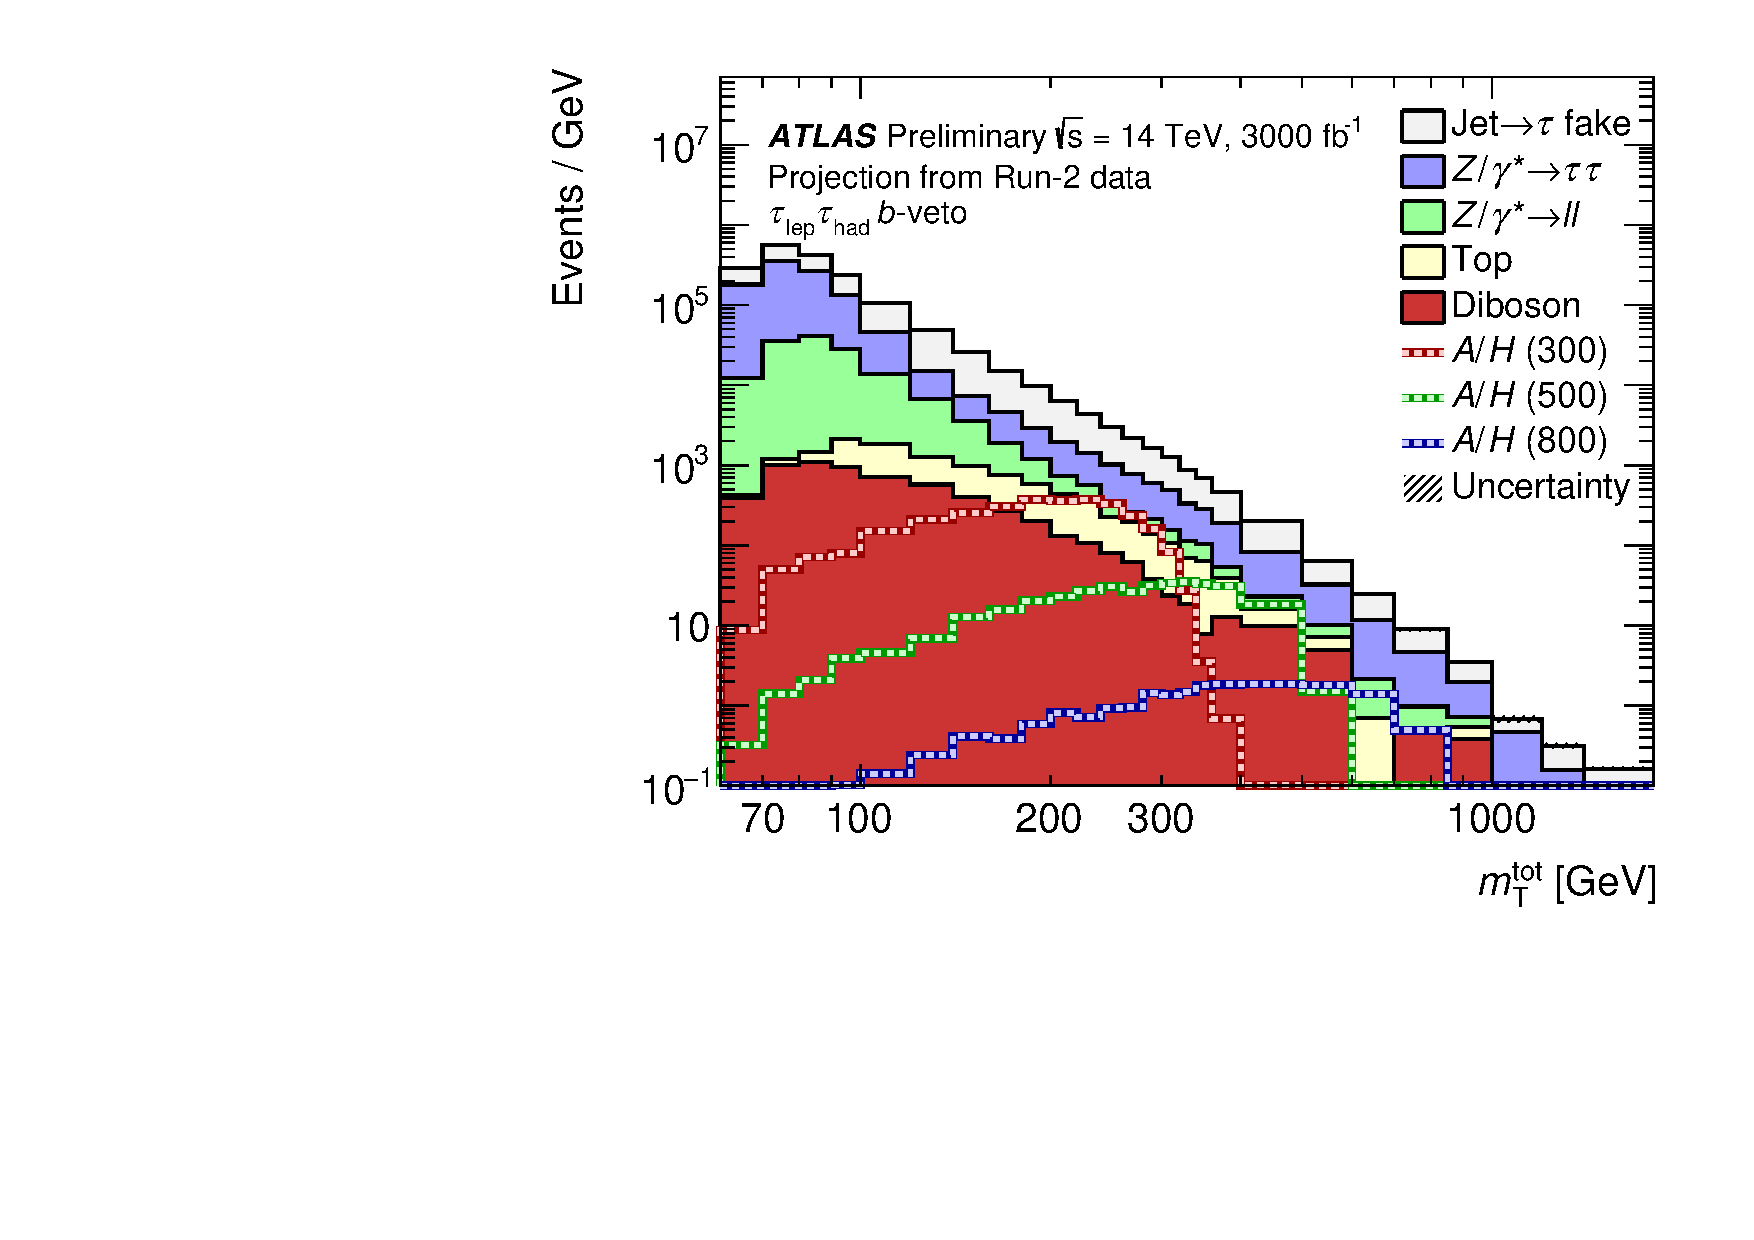
\includegraphics[width=0.45\columnwidth]{\main/section9/plots/c170_postfit_lephad_bveto_MTtot__highlumi.pdf}}
        \qquad
        \subfloat[\lephad $b$-tag category]{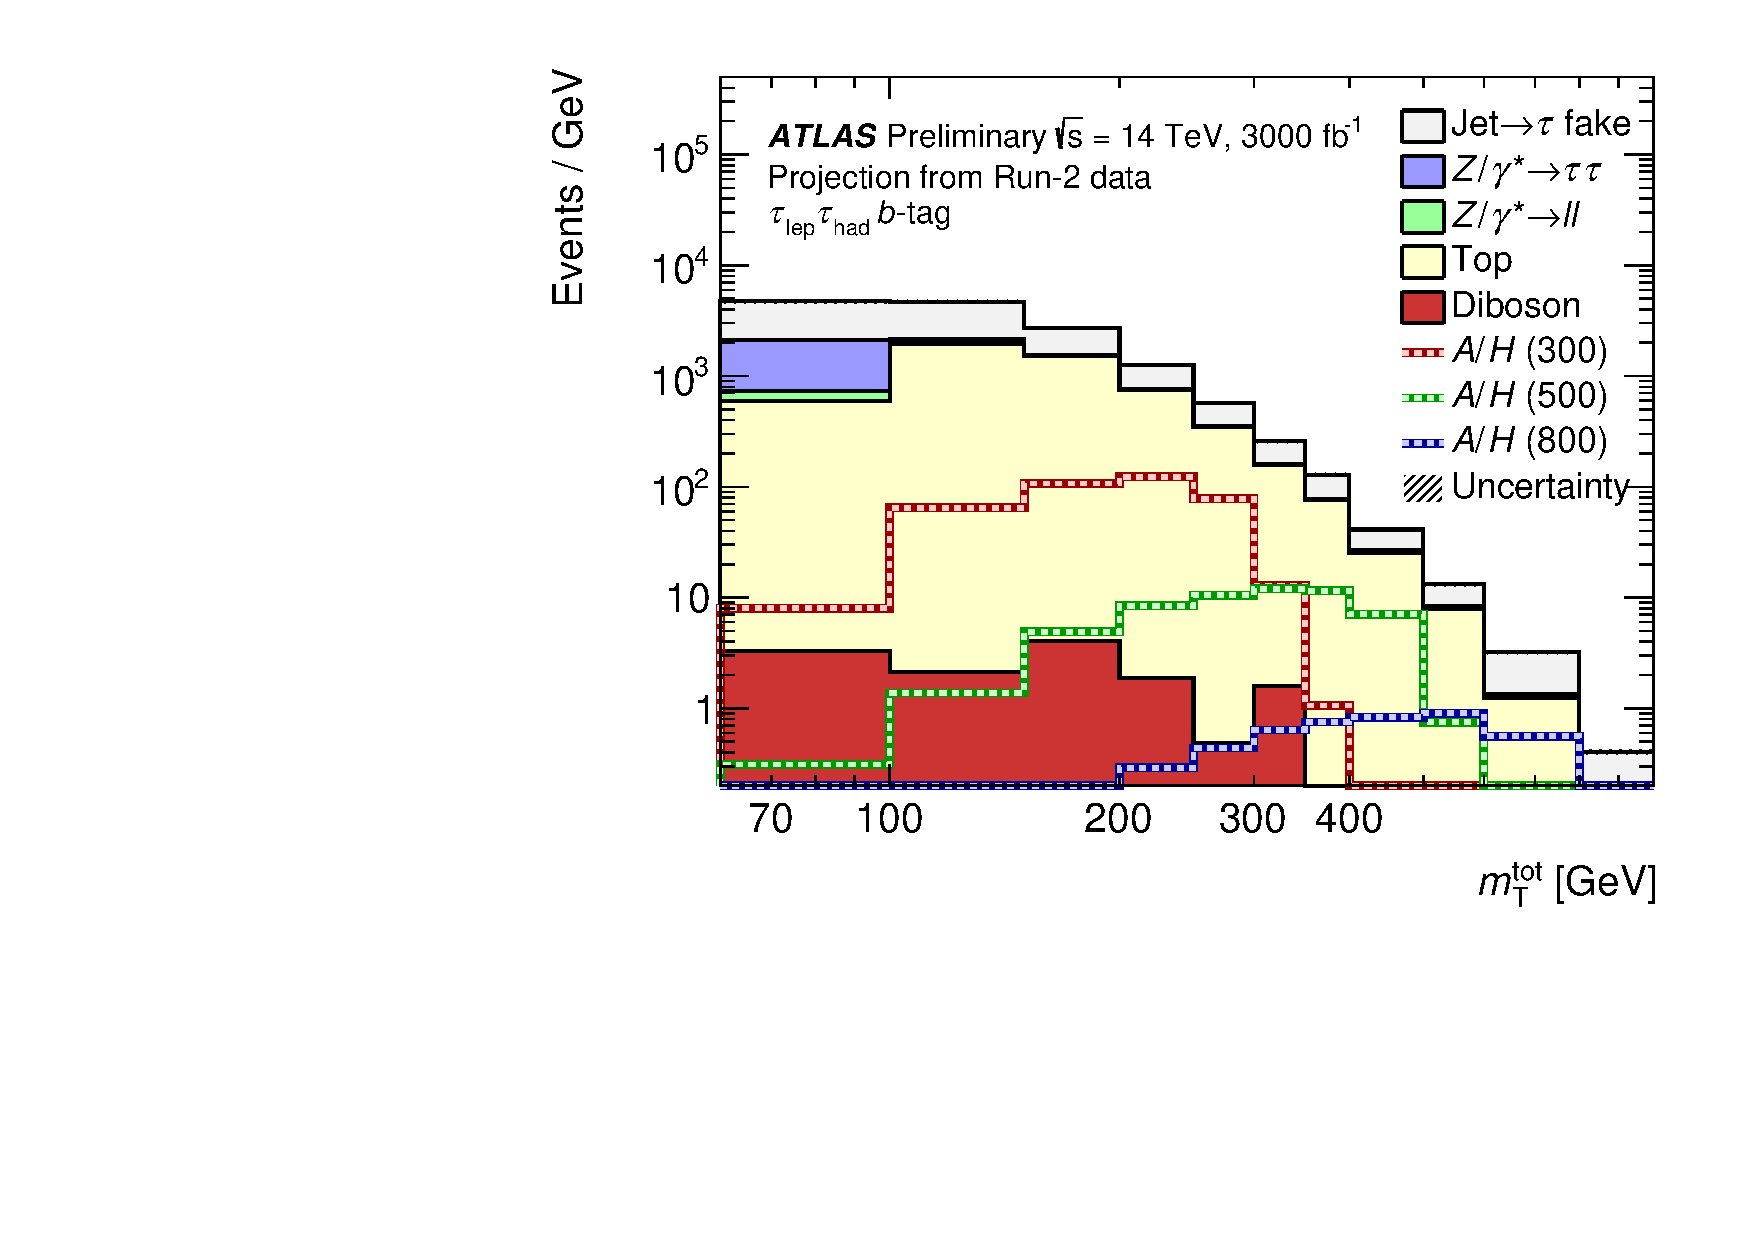
\includegraphics[width=0.45\columnwidth]{\main/section9/plots/c171_postfit_lephad_btag_MTtot__highlumi.pdf}}
        \qquad
        \subfloat[\hadhad $b$-veto category]{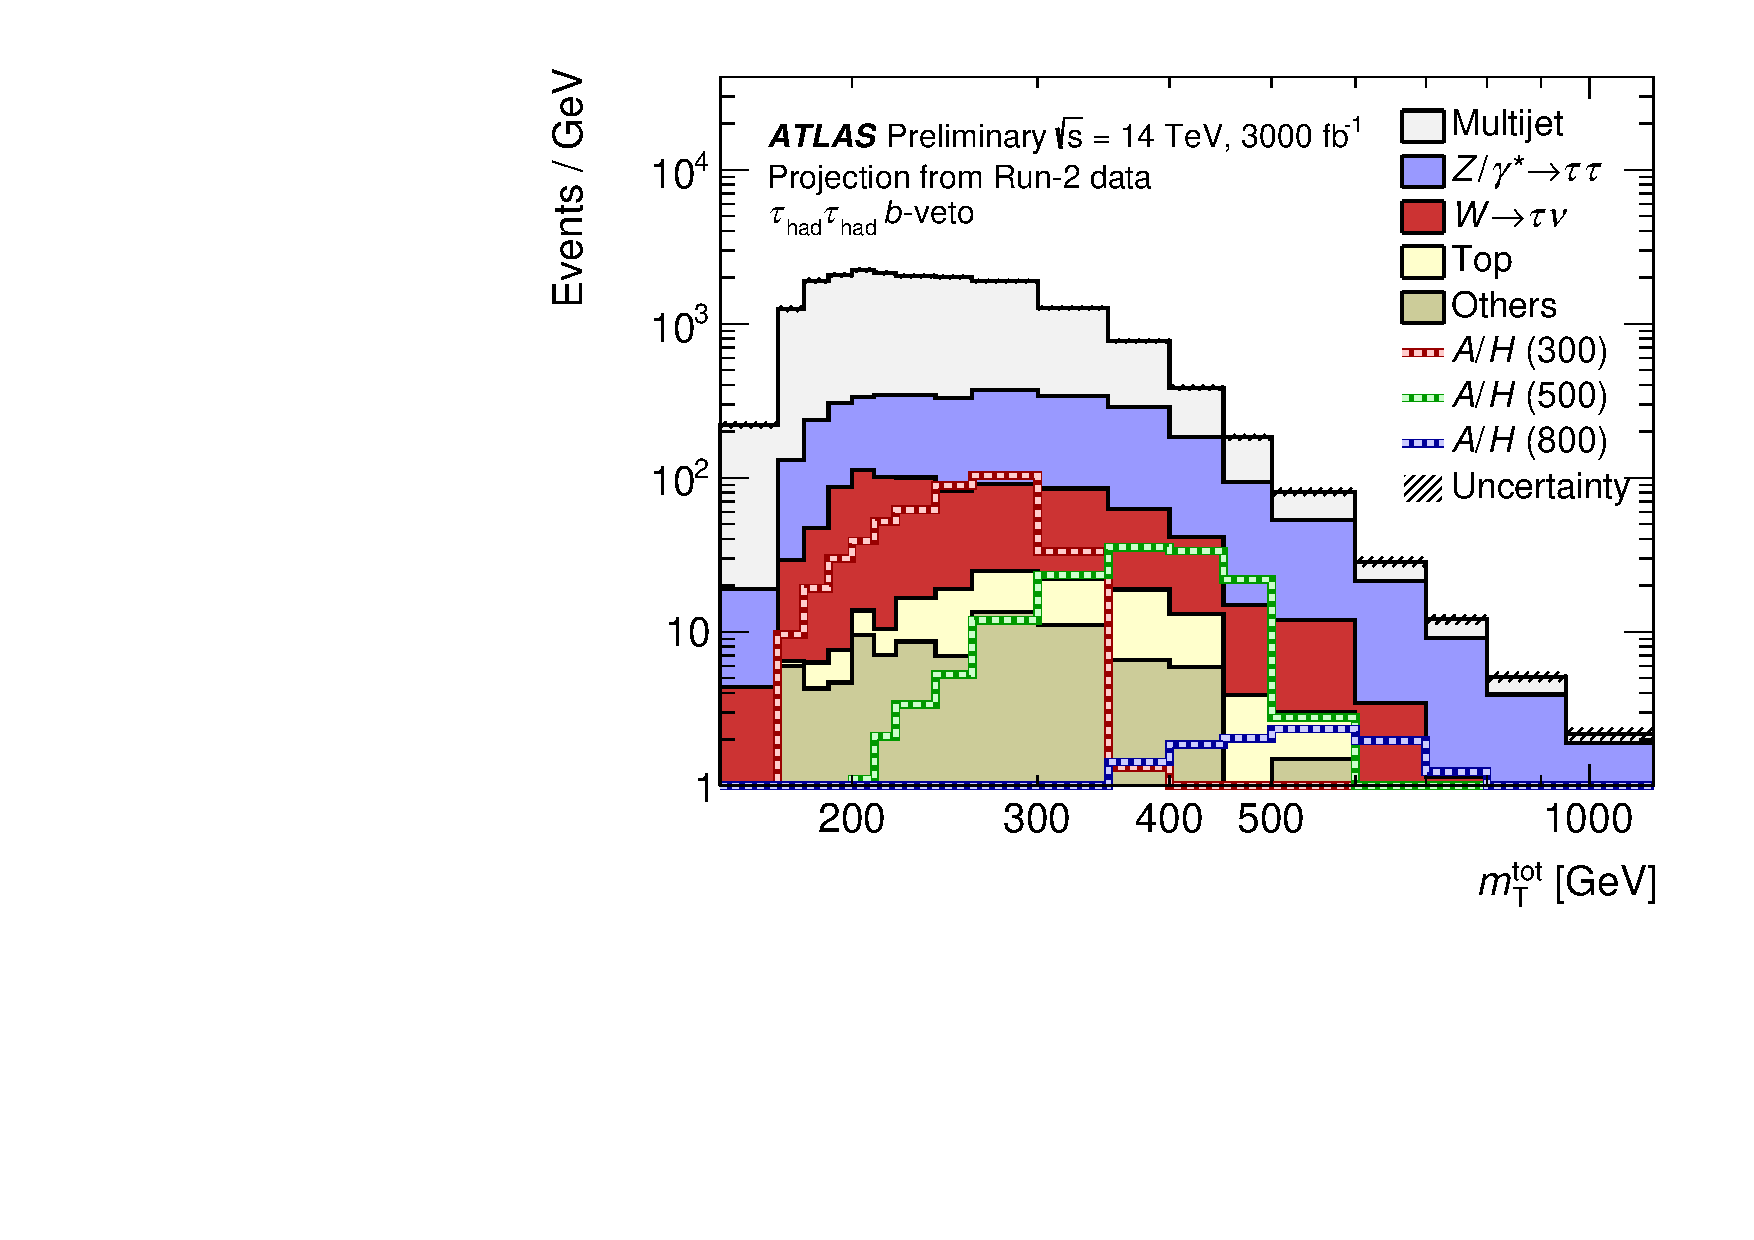
\includegraphics[width=0.45\columnwidth]{\main/section9/plots/c20_postfit_hadhad_bveto_MTtot__highlumi.pdf}}
        \qquad
        \subfloat[\hadhad $b$-tag category]{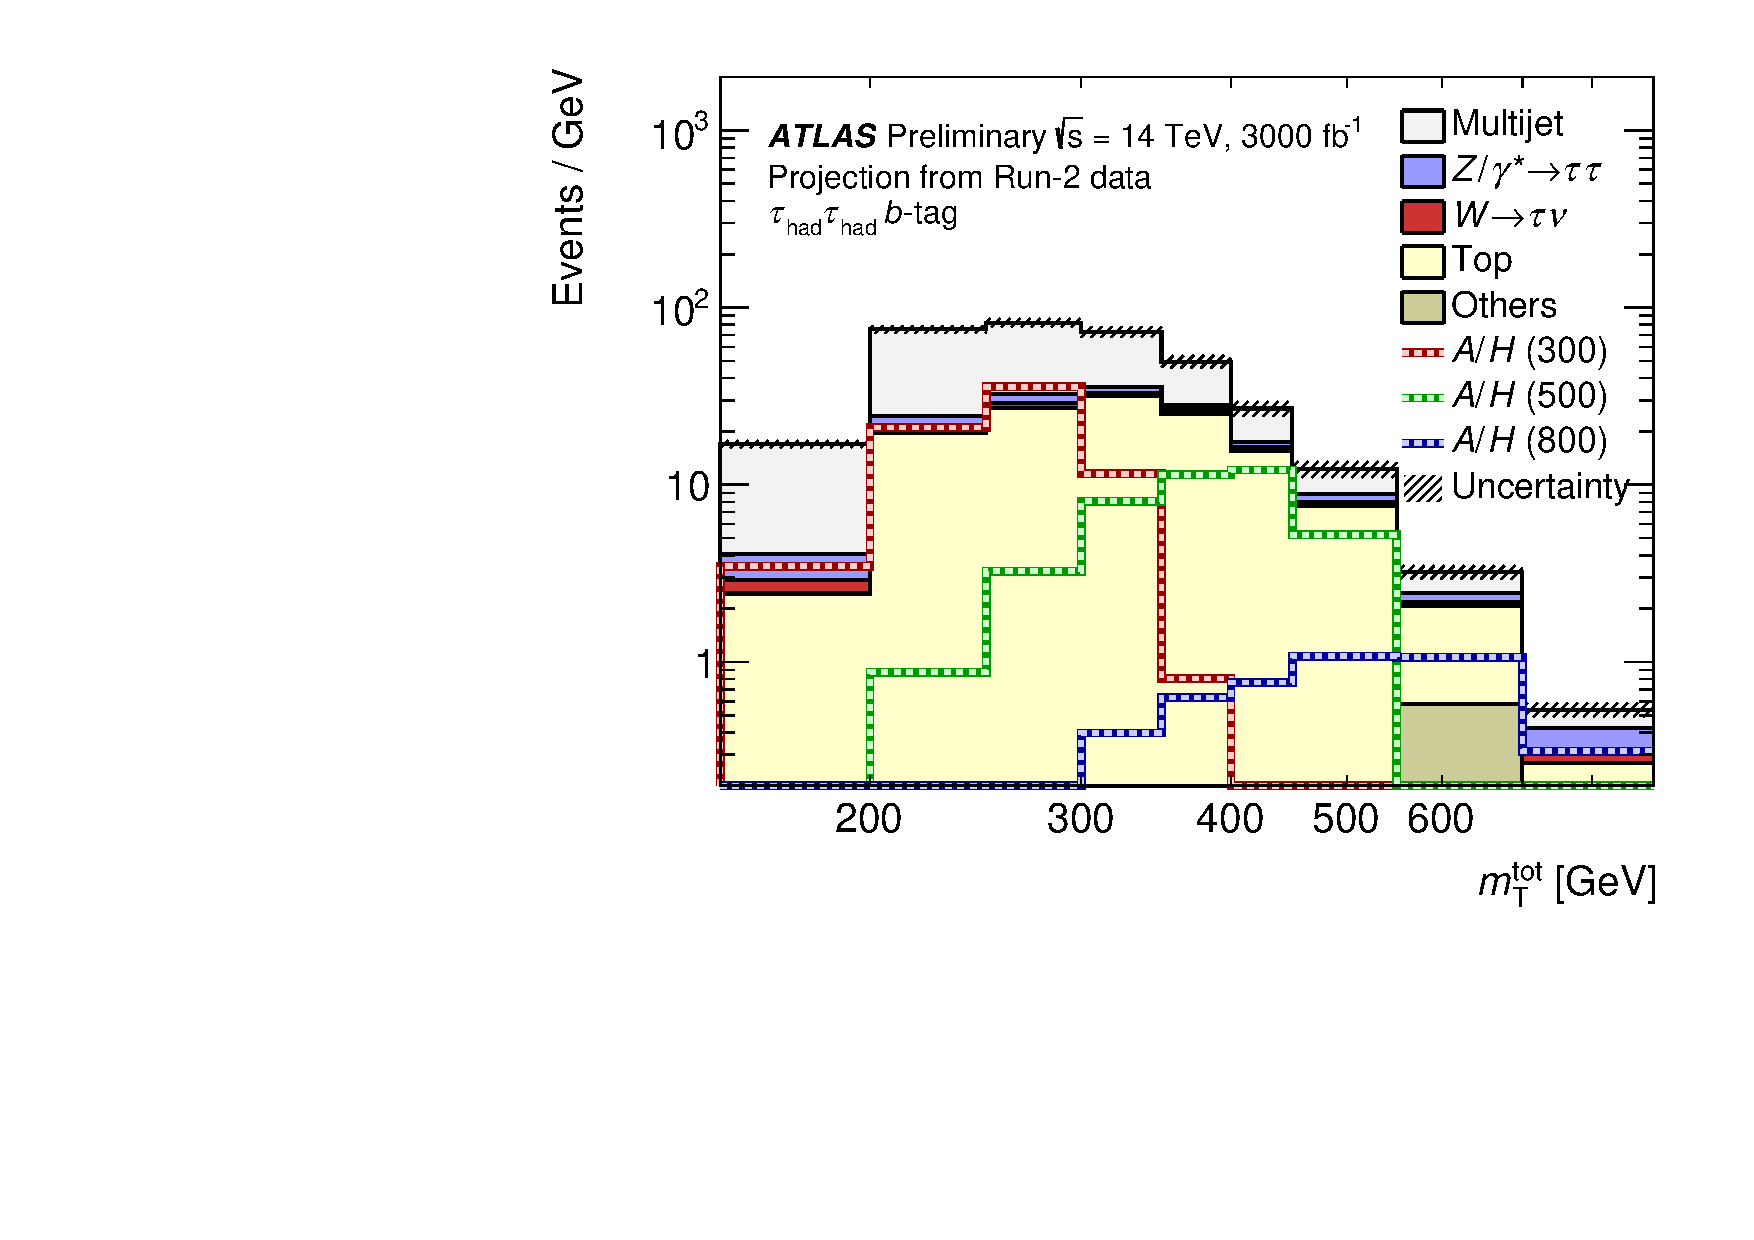
\includegraphics[width=0.45\columnwidth]{\main/section9/plots/c21_postfit_hadhad_btag_MTtot__highlumi.pdf}}
        \caption{Distributions of $\mTtot$ for each signal category. The style of the plot follows Ref.~\cite{ATLASRun2Ditau}. }

    \label{fig:mTtotDistributionsSR}
\end{figure}

\begin{figure}[!ht]
    \centering
        \qquad
        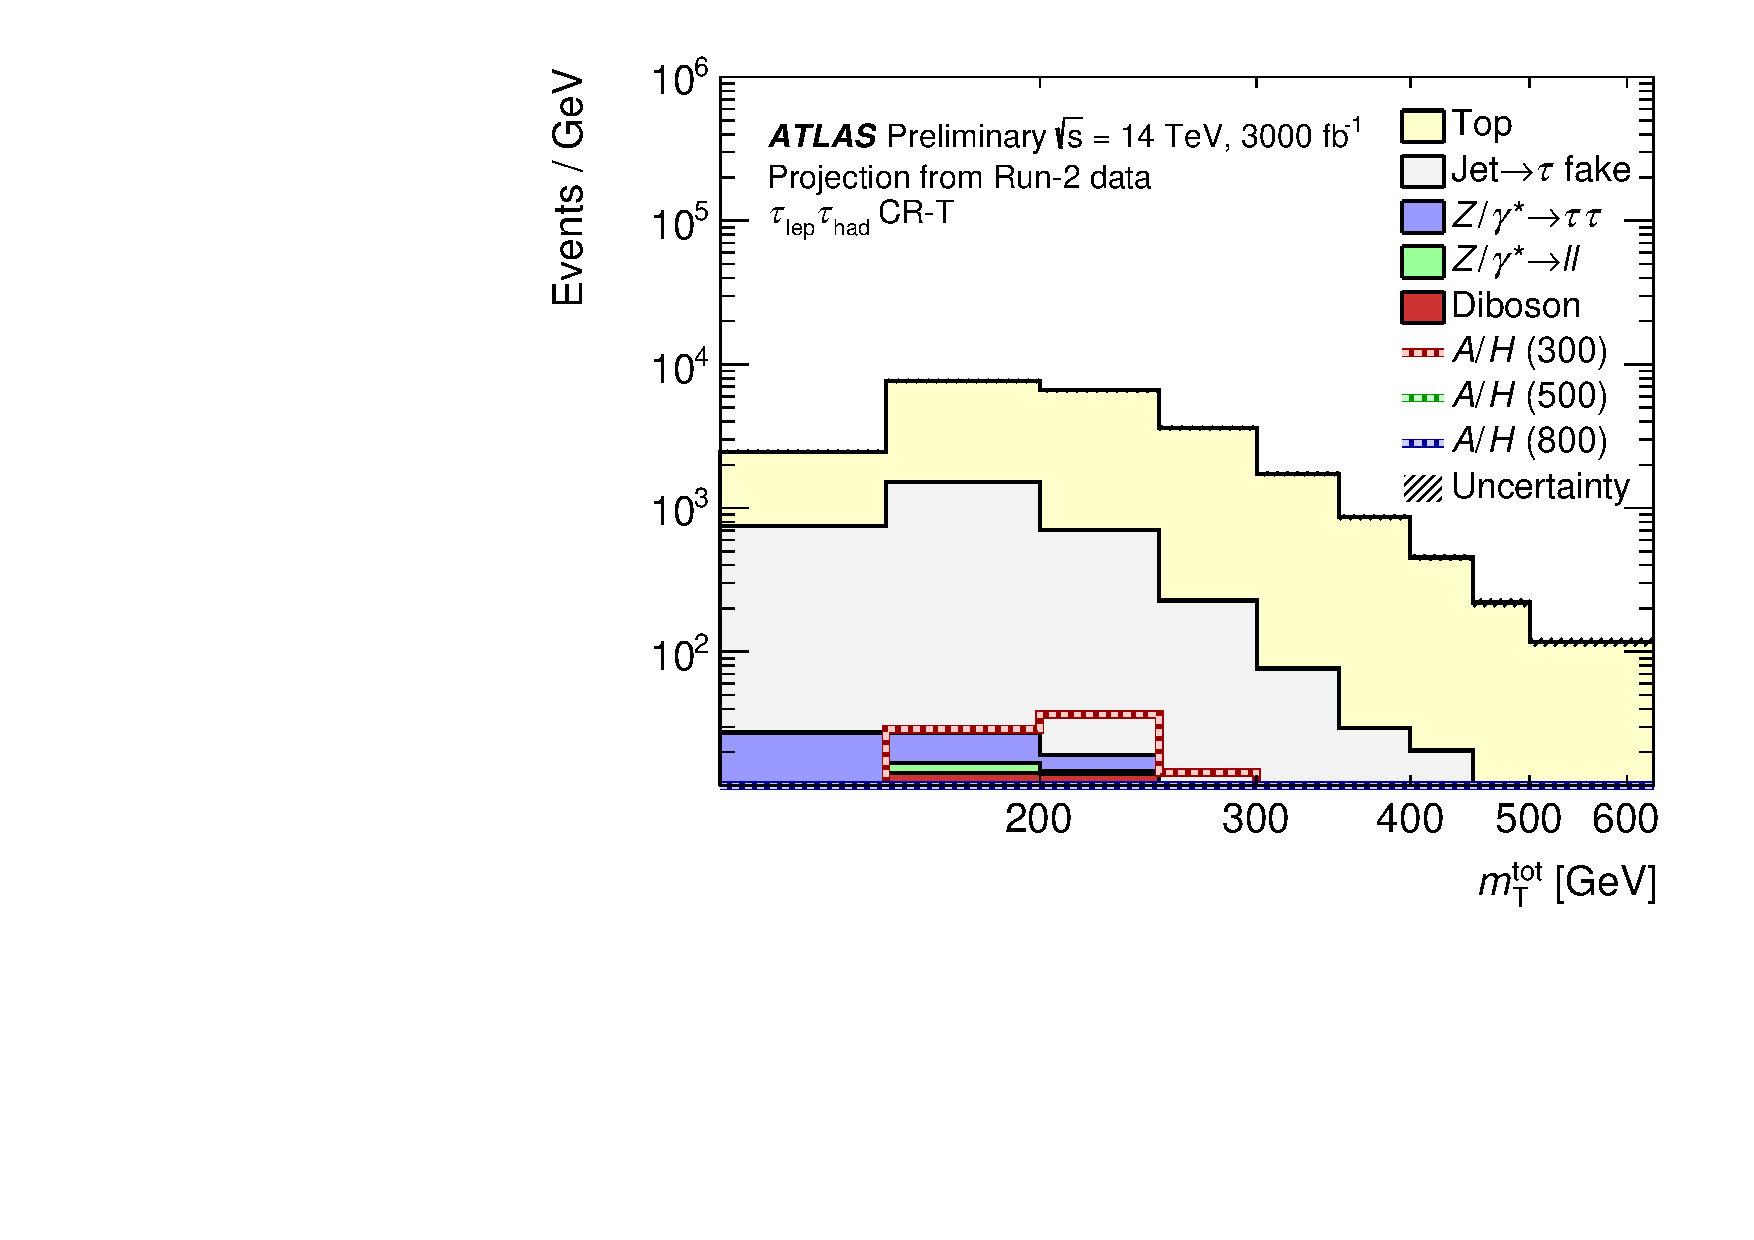
\includegraphics[width=0.5\columnwidth]{\main/section9/plots/c181_postfit_lephad_tcr_MTtot__highlumi.pdf}
        \caption{Distribution of $\mTtot$ distributions in in the top quark enriched control region of the \lephad channel.}
    \label{fig:mTtotDistributionsCR}
\end{figure}

With the larger dataset at HL-LHC, the systematic uncertainties in this analysis are expected to be reduced.
The systematic uncertainties associated with $b-$tagging, $\tauhadvis$ and theoretical uncertainties due to 
the missing higher order calculation, the PDF uncertainty, etc. are are reduced according to 
Ref. \cite{LHATLASdetectorSystScale}. The systematic uncertainties associated with the reconstruction 
and identification of the high-$\pt$~$\tauhadvis$ is reduced by a factor of 2 and is the dominant 
uncertainty for a heavy Higgs boson with mass $m_{\phi} >\SI{1}{\UTeV}$. The systematic uncertainty associated 
with the modeling of the jet to $\tauhadvis$ fake background is assumed to be the same as the current analysis.
For the multijet background in \hadhad channel, where the modeling of the jet to $\tauhadvis$ fake background 
is limited by the data sample size in the control region, this uncertainty is reduced by a factor of 2. 
The statistical uncertainties of the predicted signal and background distributions is determined 
by the size of the MC samples and the data sample in the failed \tauhadvis identification control region 
(CR-1 in ~\cite{ATLASRun2Ditau}). The impact of this statistical uncertainty is negligible in the Run 2 analysis. 
Assuming enough MC samples will be generated in HL-LHC, the uncertainties due to 
the sample size is ignored in this extrapolation study. The theoretical uncertainties, e.g. the signal acceptance 
uncertainties due to the missing higher order calculation, the PDF uncertainty, etc., are also assumed to be 
the same. The uncertainties associated to $e$, $\mu$, jet, $\mathrm{E^{miss}_T}$ have minor impact to the analysis 
and are assumed to be the same for simplicity. This systematic uncertainty treatment scheme is defined as ``Baseline''. 

The statistical framework used to produce the Run-2 results is documented in Ref.~\cite{ATLASRun2Ditau} is adapted 
for this HL-LHC projection study. A likelihood function constructed as the product of Poisson probability terms 
is used. A term is included for each bin in the $\mTtot$ distributions from the \lephad and \hadhad signal regions, 
as well as the top control region. 

%-------------------------------------------------------------------------------
\paragraph{Results}
\label{sec:result}

Assuming the data are found to be in good agreement with the predicted background, the results 
are given in terms of exclusion limits \cite{CLs_2002}. 

%-------------------------------------------------------------------------------
%\paragraph{Impact of systematic uncertainties}
%The impact of systematic uncertainties on the model-independent $\phi\to\tau\tau$ upper limits are calculated 
%by comparing the expected 95\% CL upper limit in case of no systematic uncertainties, $\mu^{95}_{\text{stat}}$, 
%with a limit calculated by introducing a group of systematic uncertainties, $\mu^{95}_i$, as described 
%in Ref. \cite{ATLASRun2Ditau}. The systematic uncertainty impacts are shown in Figure \ref{fig:sysimpact} (a) 
%for $\mathrm{ggf}$ production and Figure \ref{fig:sysimpact} (b) for $\mathrm{bb\phi}$ production as functions of 
%the scalar boson mass.  The major uncertainties are grouped according to their origin, while minor uncertainties 
%are collected as ``Others''.

%It can be seen that the systematic uncertainty is crucial in the whole search range.
%In the low mass range, the major uncertainties arise from the estimate of the dominant jet to $\tauhadvis$ 
%fake background. At high masses, the dominant uncertainty for ggf is from the reconstruction and identification 
%for high-$\pt$~ $\tauhadvis$, while for $\mathrm{bb\phi}$ the $b$-tagging related uncertainty is also important. 
%In Figure \ref{fig:sysimpact} (a), the peak structure at $\SI{1}{\UTeV}$ 
%of the $\tauhadvis$ related systematic uncertainties is due to the complicated interaction 
%between the signal shape and systematic uncertainty variations in the combined likelihood fit.

%\begin{figure}[!ht]
%    \centering
%        \subfloat[gluon--gluon fusion production]{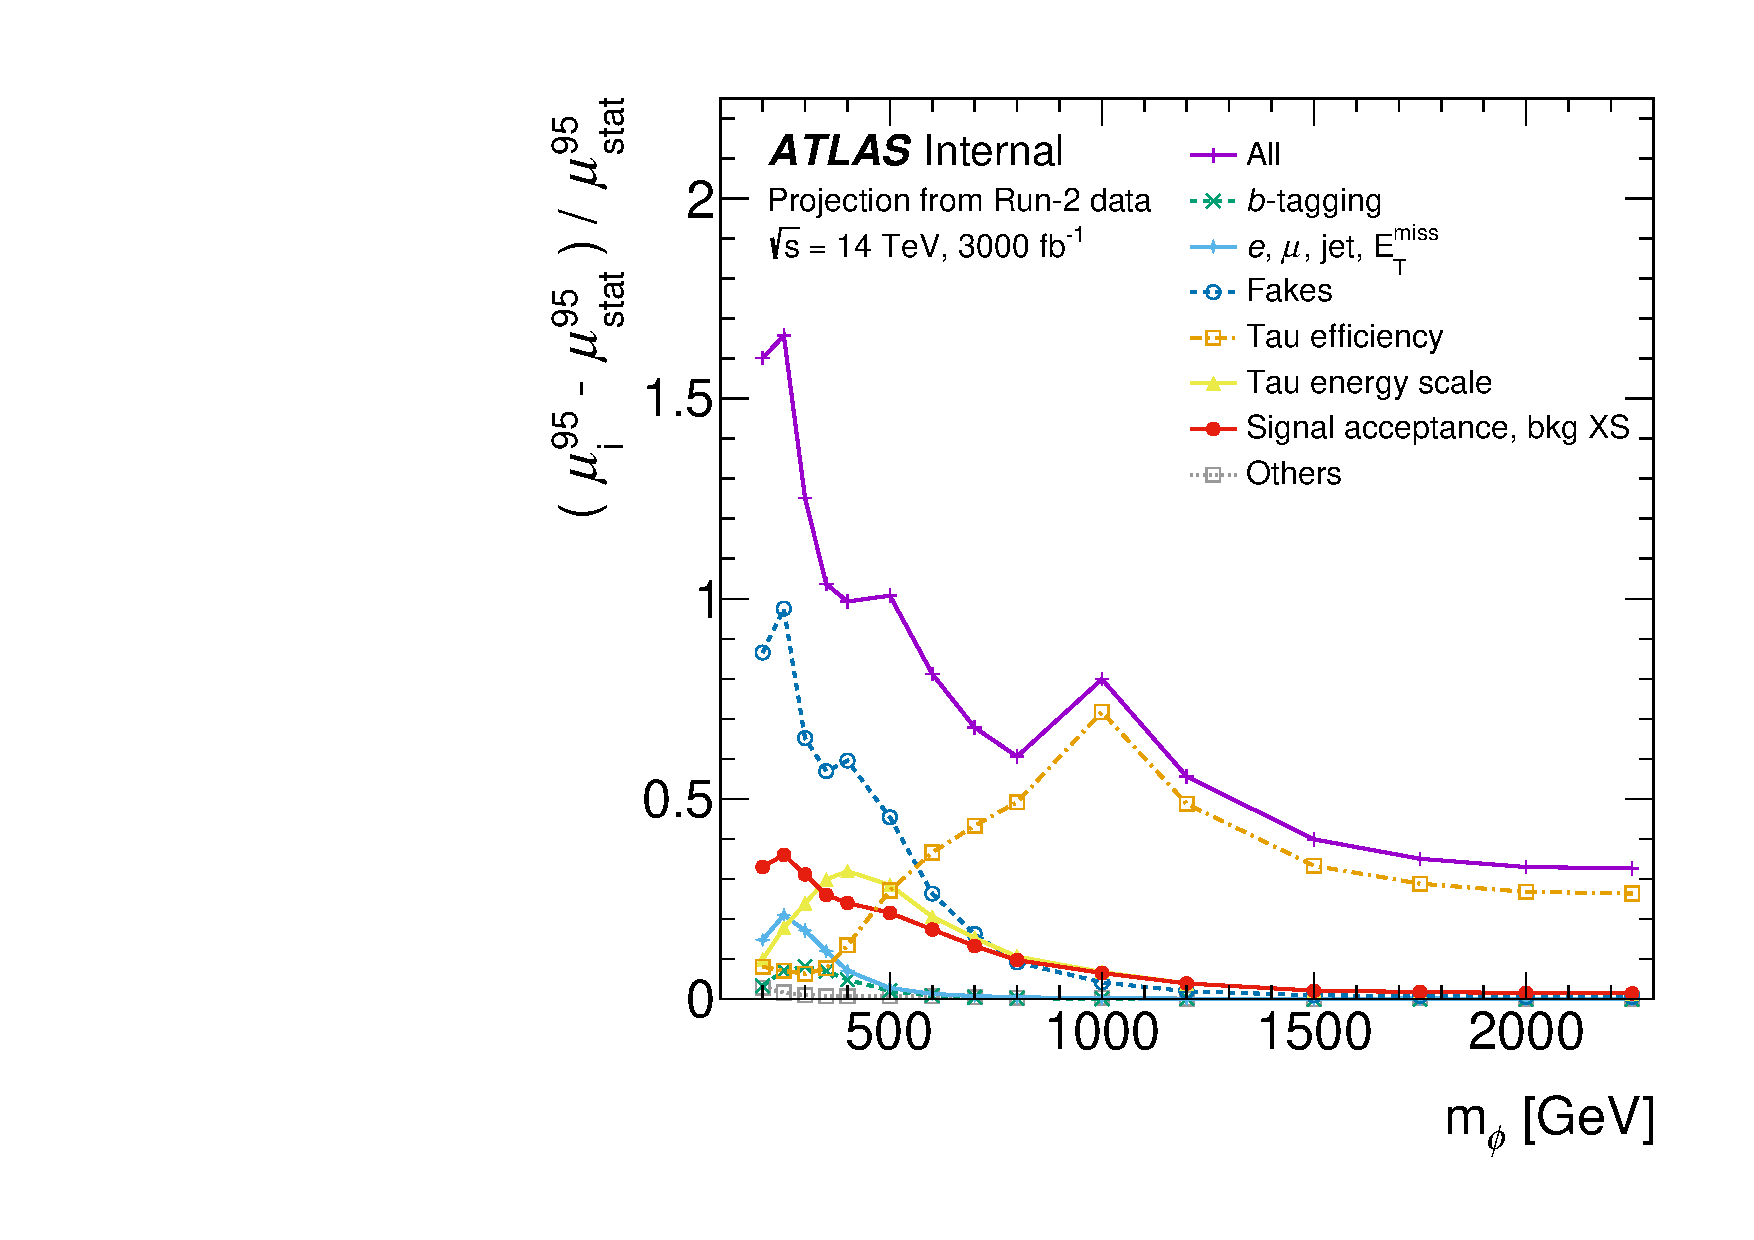
\includegraphics[width=0.4\columnwidth]{\main/section9/plots/ggH__syst_impacts.pdf}}
 %       \qquad
%        \subfloat[$b$-associated production]{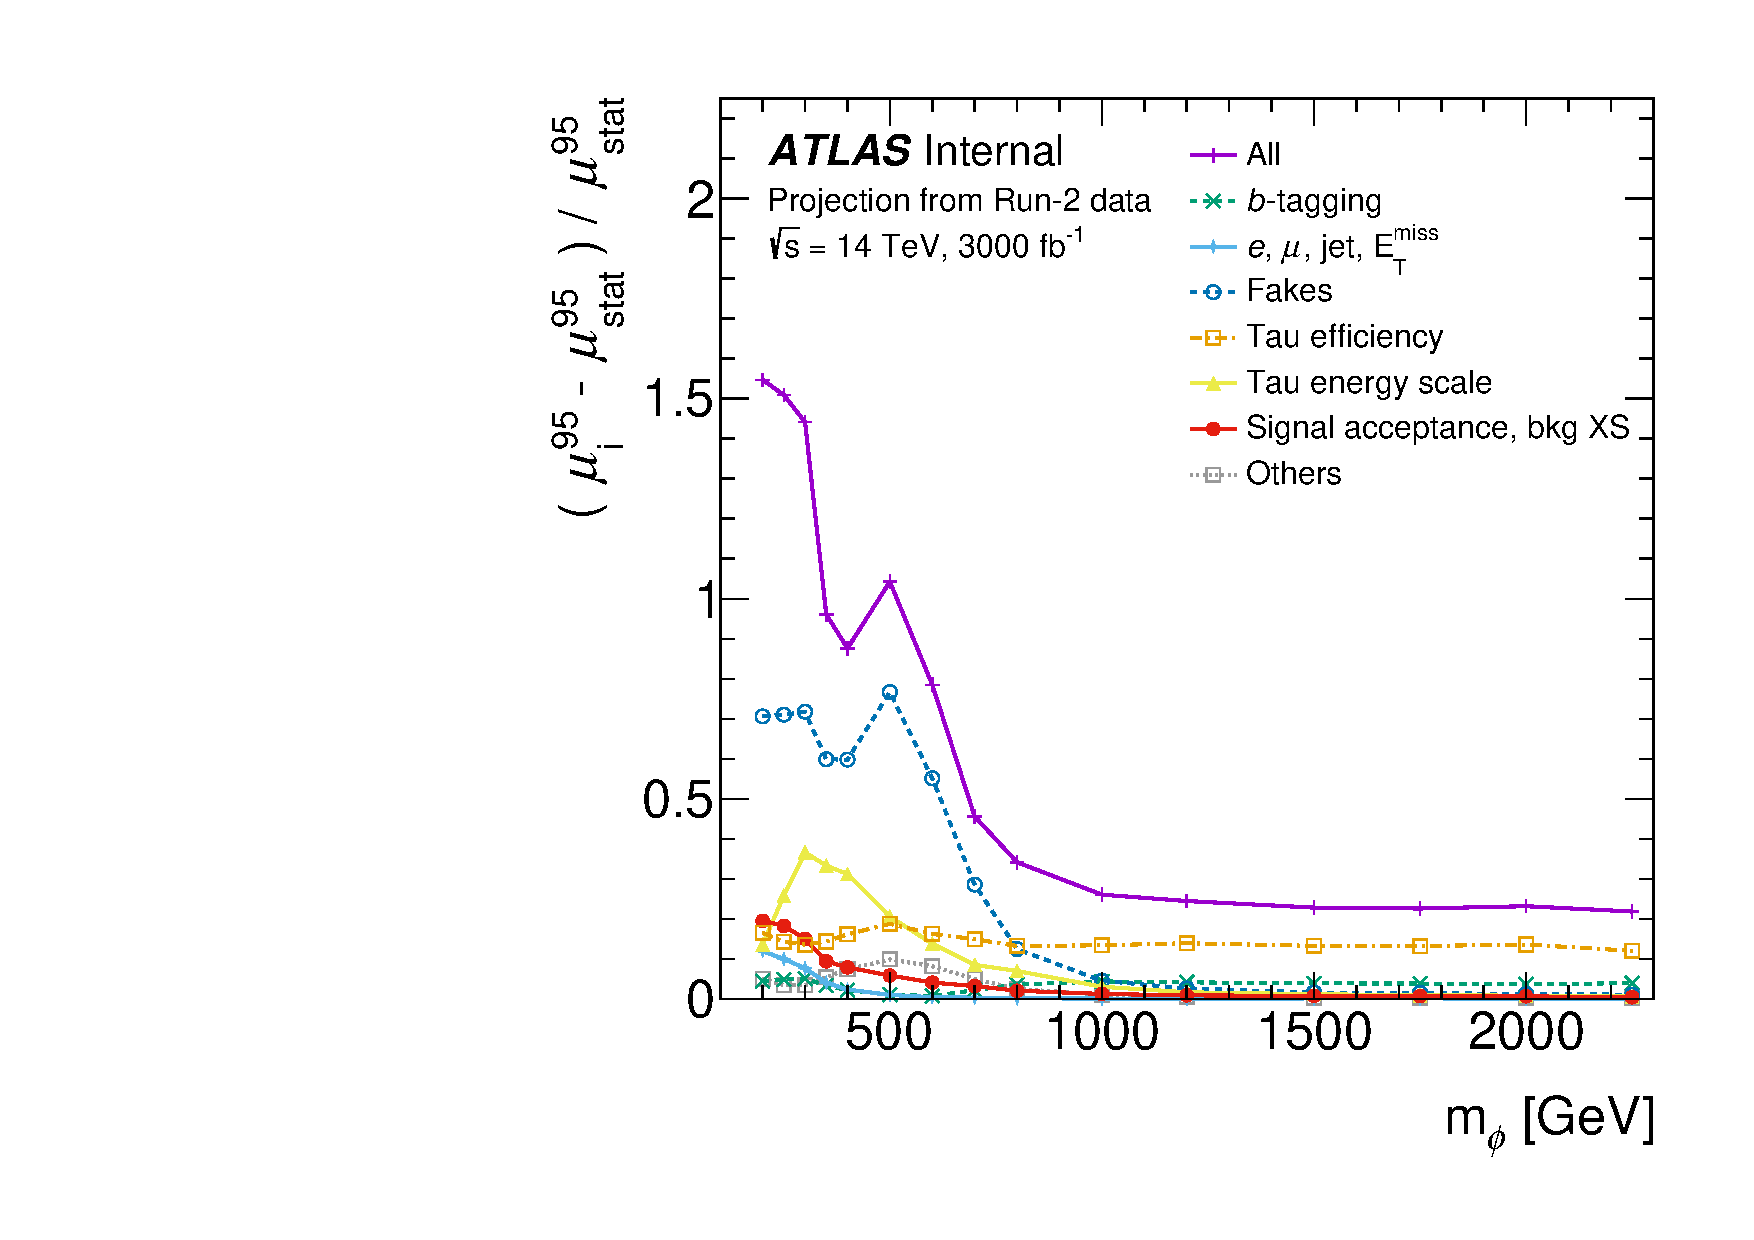
\includegraphics[width=0.4\columnwidth]{\main/section9/plots/bbH__syst_impacts.pdf}}
%        \caption{Impact of major groups of systematic uncertainties on the $\phi\to\tau\tau$ 95\% CL 
%          cross section upper limits as a function of the scalar boson mass, separately 
%          for the (a) gluon--gluon fusion and (b) $b$-associated production mechanisms.}
%    \label{fig:sysimpact}
%\end{figure}

\paragraph{Cross section limits}
Figure \ref{fig:modelInde} shows the upper limits on the gluon--gluon fusion and $b$-quark associated production 
cross section times ditau branching fraction. To demonstrate the impact of systematics, the expected exclusion limits
with different systematic uncertainty schemes are shown, as well as the current Run 2 results\cite{ATLASRun2Ditau}.
The peaking structure around $m_\phi = 1$ TeV in figure \ref{fig:modelInde} (a) is due to the impact of 
the high-$\pt$ tau systematic uncertainty. 

\begin{figure}[!ht]
    \centering
        \subfloat[gluon--gluon fusion production]{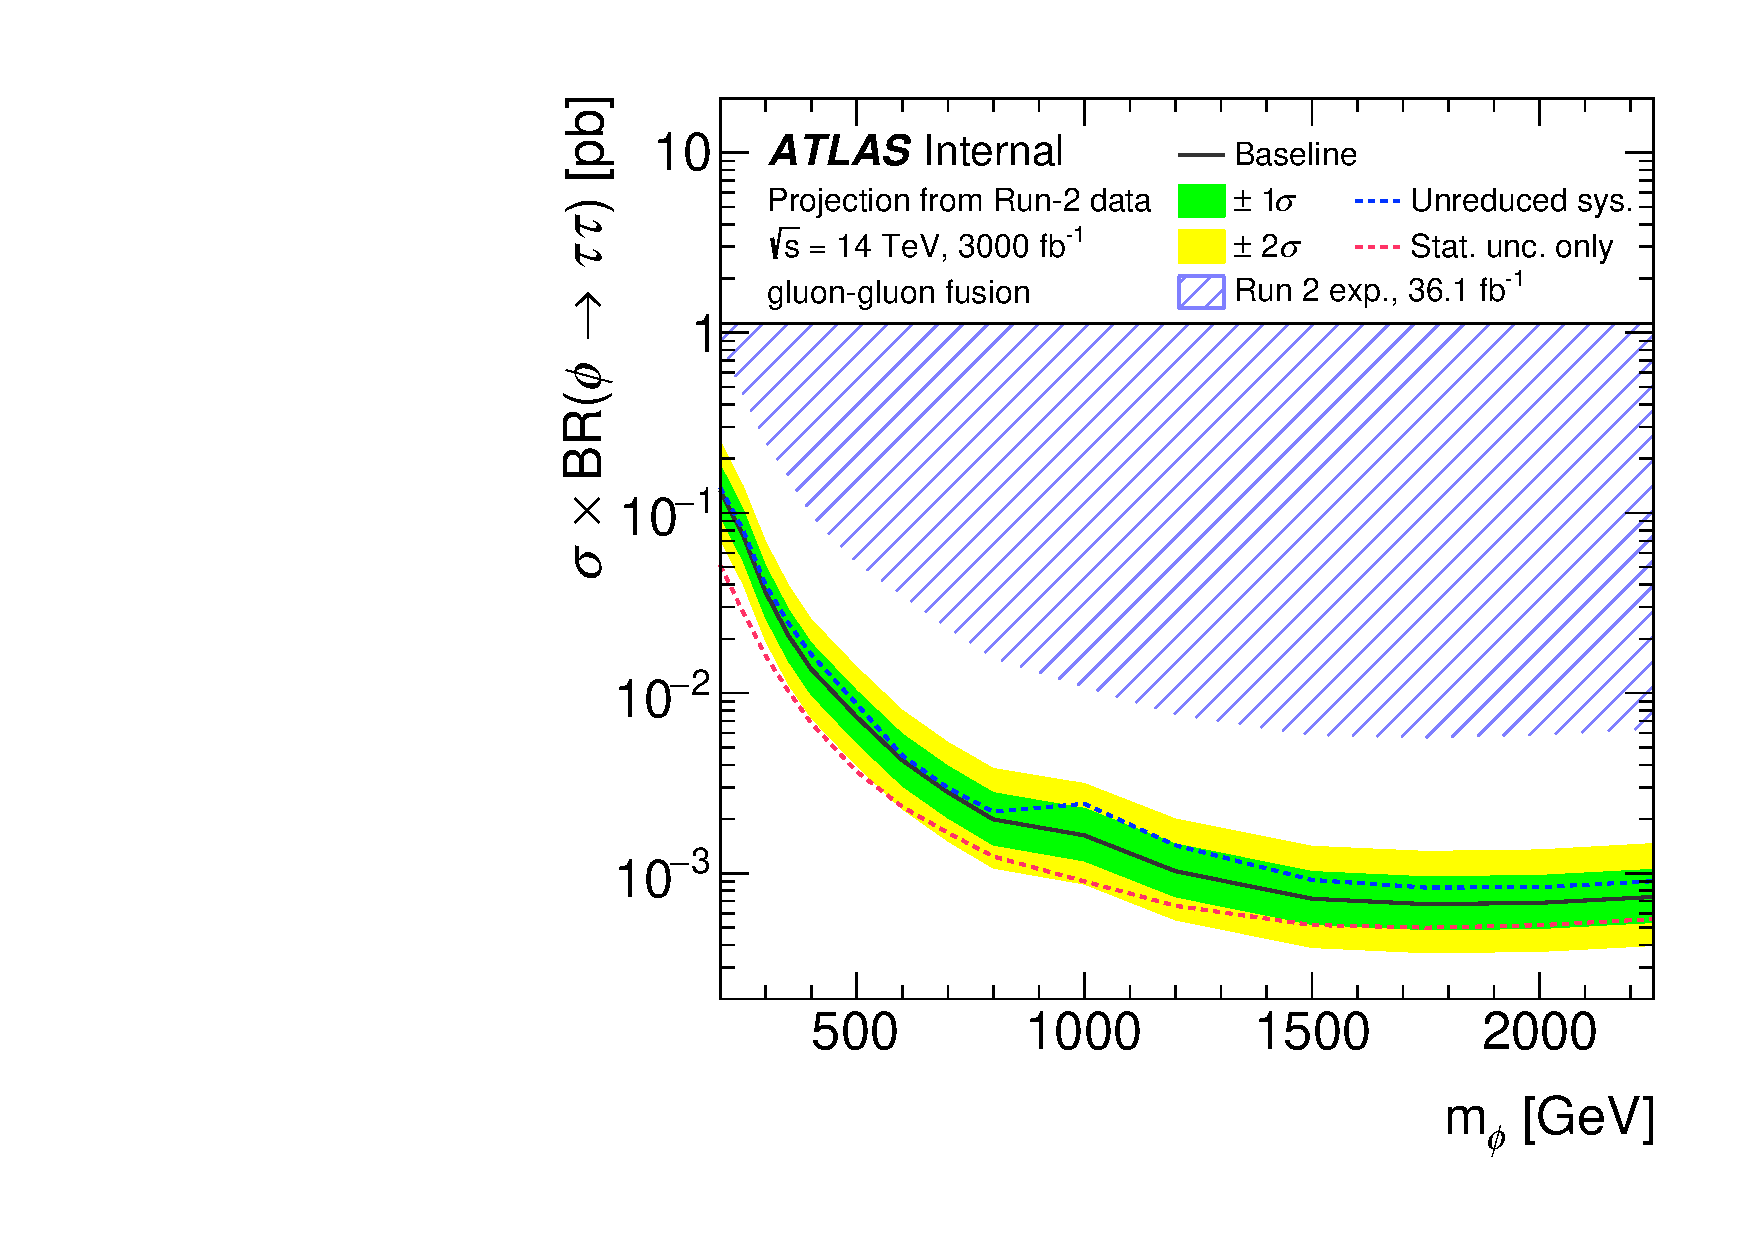
\includegraphics[width=0.4\columnwidth]{\main/section9/plots/ggH.pdf}}
        \qquad
        \subfloat[$b$-associated production]{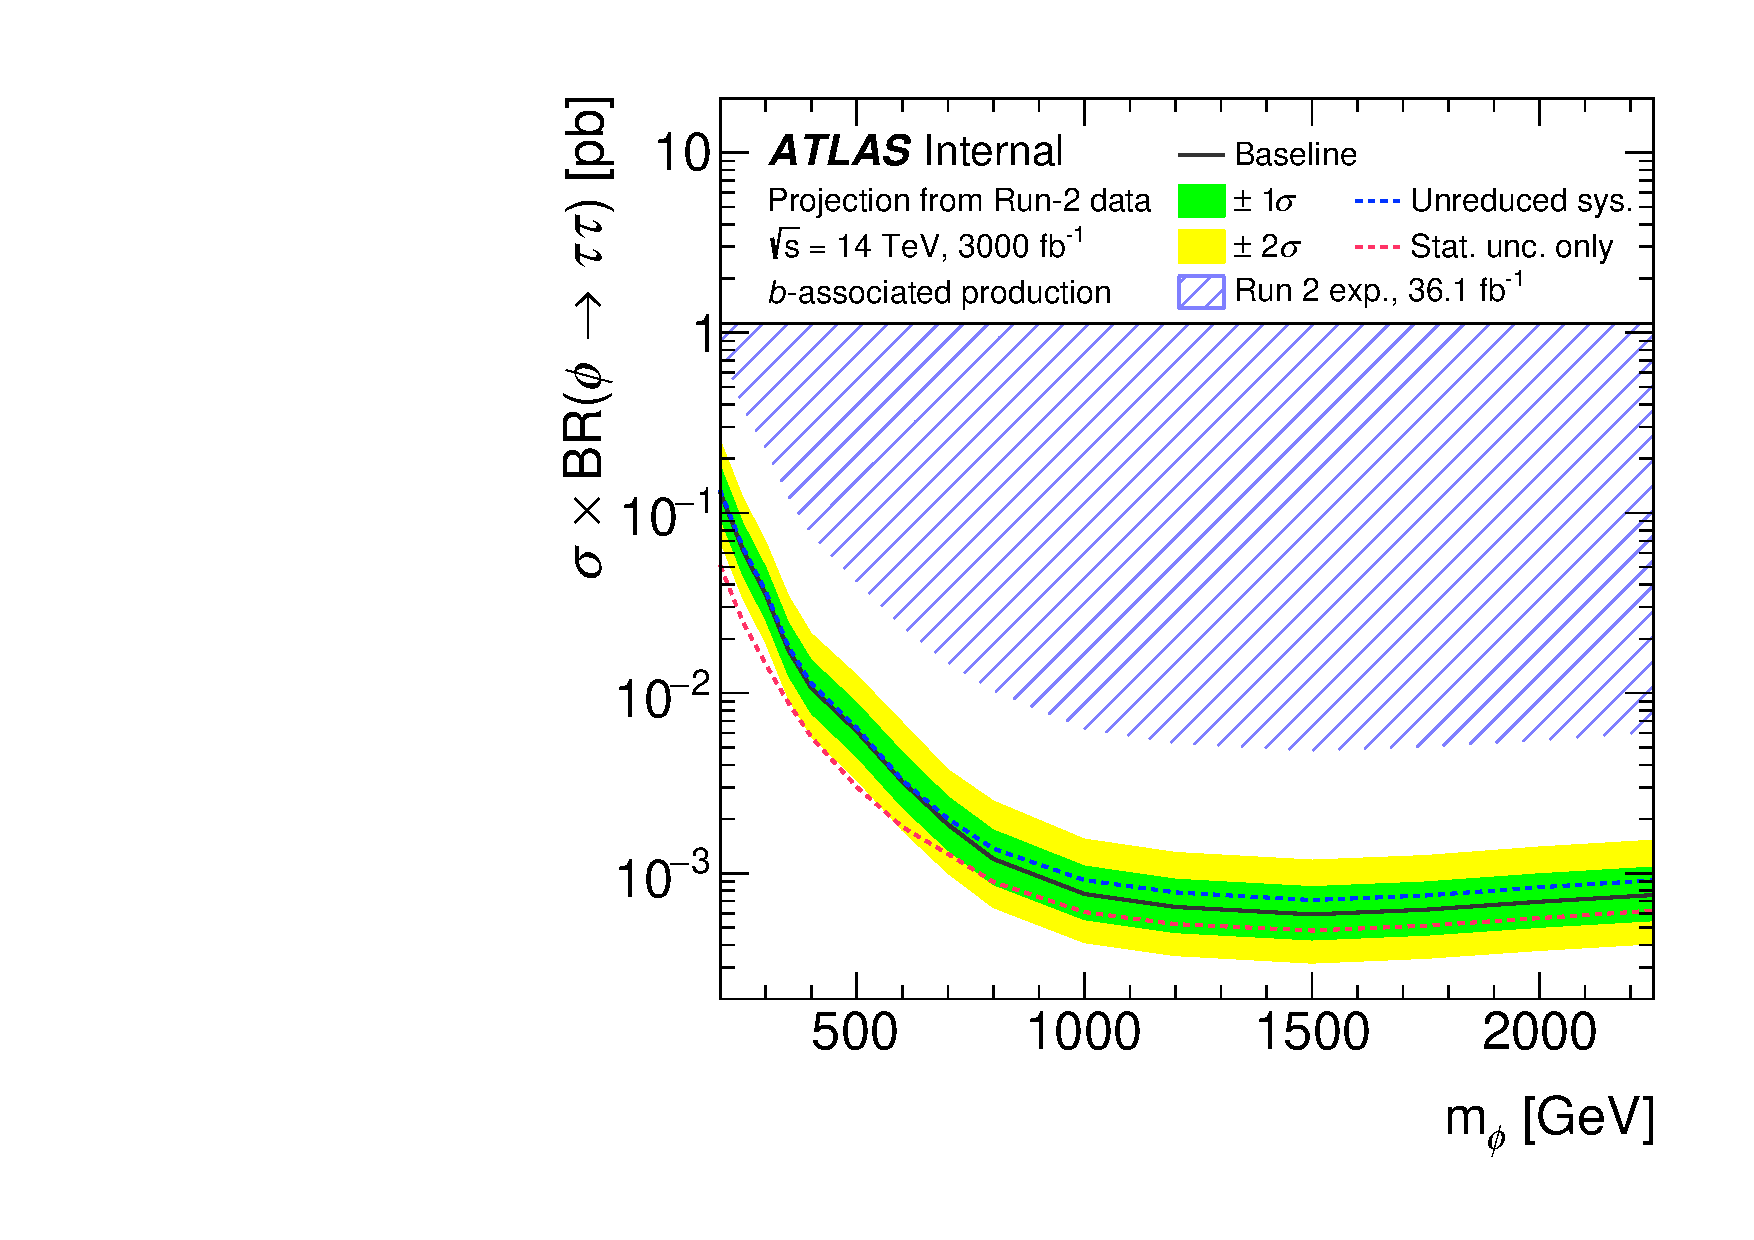
\includegraphics[width=0.4\columnwidth]{\main/section9/plots/bbH.pdf}}
        \caption{Projected 95\% CL upper limits on the production cross section times ditau branching fraction 
        for a scalar boson produced via (a) gluon--gluon fusion and (b) $b$-associated production, as a function 
        of scalar boson mass. The limits are calculated from a statistical combination of the \ehad, \muhad 
        and \hadhad channels. ``Baseline'' uses the reduced systematic uncertainties scheme described in the text.
        ``Unreduced sys.'' uses the same systematic uncertainties as the Run 2 analysis while ignoring 
        the statistical uncertainty due to the limited data size of the signal and backgrounds. 
        ``Stat. unc. only'' represents the expected limit without considering any systematic uncertainty.
        }
    \label{fig:modelInde}
\end{figure}

\paragraph{MSSM interpretation}
Results are interpreted in terms of the MSSM. Figure \ref{fig:model1} shows regions in the $m_\phi-\tan\beta$ 
plane excluded at 95\% CL in the hMSSM and $m_{h}^{\text{mod}+}$ scenarios. In the hMSSM scenario, 
$\tan\beta >$~1.0 for $m_\phi < 350$ GeV and $\tan\beta >$~15 for $m_\phi = 1.5$ TeV can be excluded at 95\% CL. 
When $m_\phi$ is above the $\phi\to$\ttbar threshold, this additional decay mode reduces the sensitivity 
of the $A\to\tau\tau$ search for low $\tan\beta$. In the MSSM $m_{h}^{\text{mod}+}$ scenario, 
the expected 95\% CL upper limits exclude $\tan\beta >1$ for $m_\phi< 350$ GeV and $\tan\beta >$ ~ 25 
for $m_\phi = 1.5$ TeV.

\begin{figure}[!ht]
    \centering
        \subfloat[hMSSM scenario]{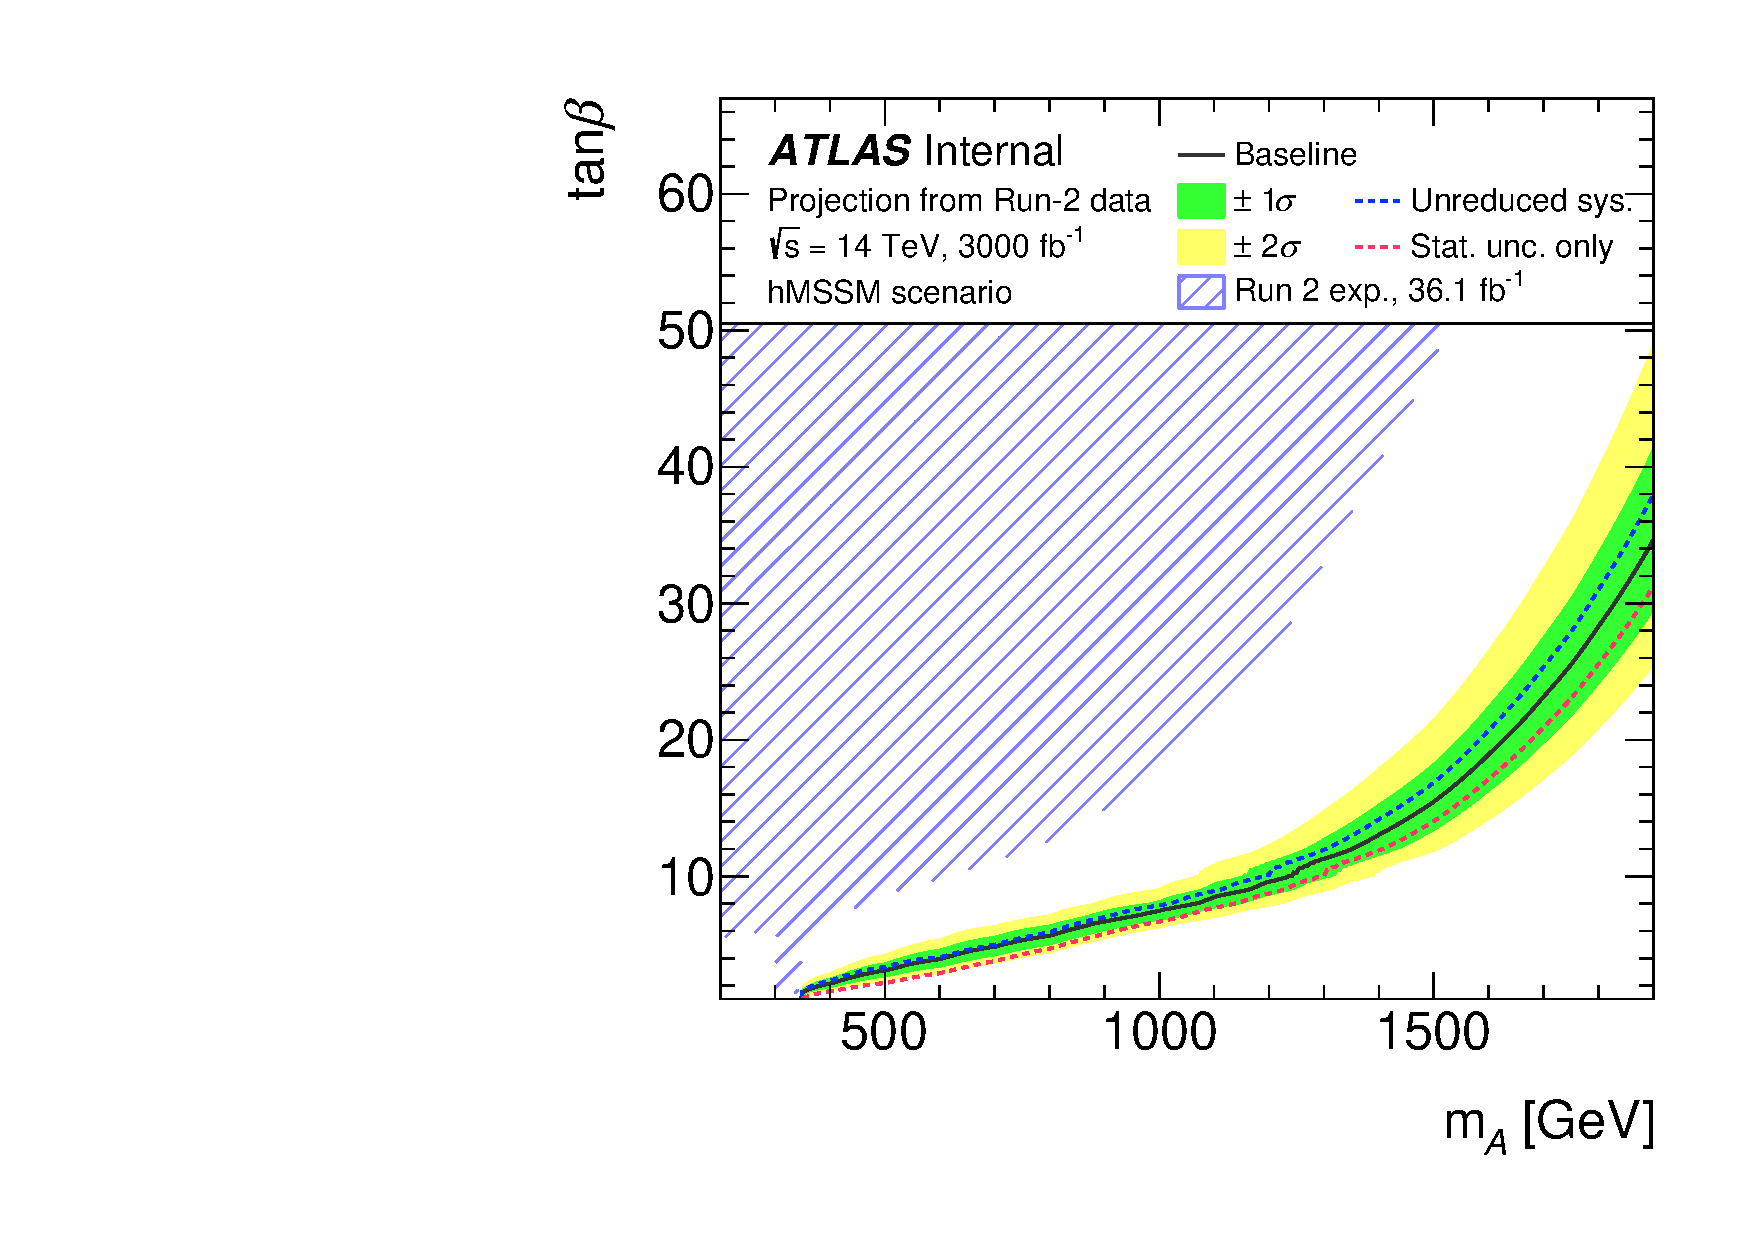
\includegraphics[width=0.4\columnwidth]{\main/section9/plots/hMSSM.pdf}}
        \qquad
        \subfloat[\mhmodp scenario]{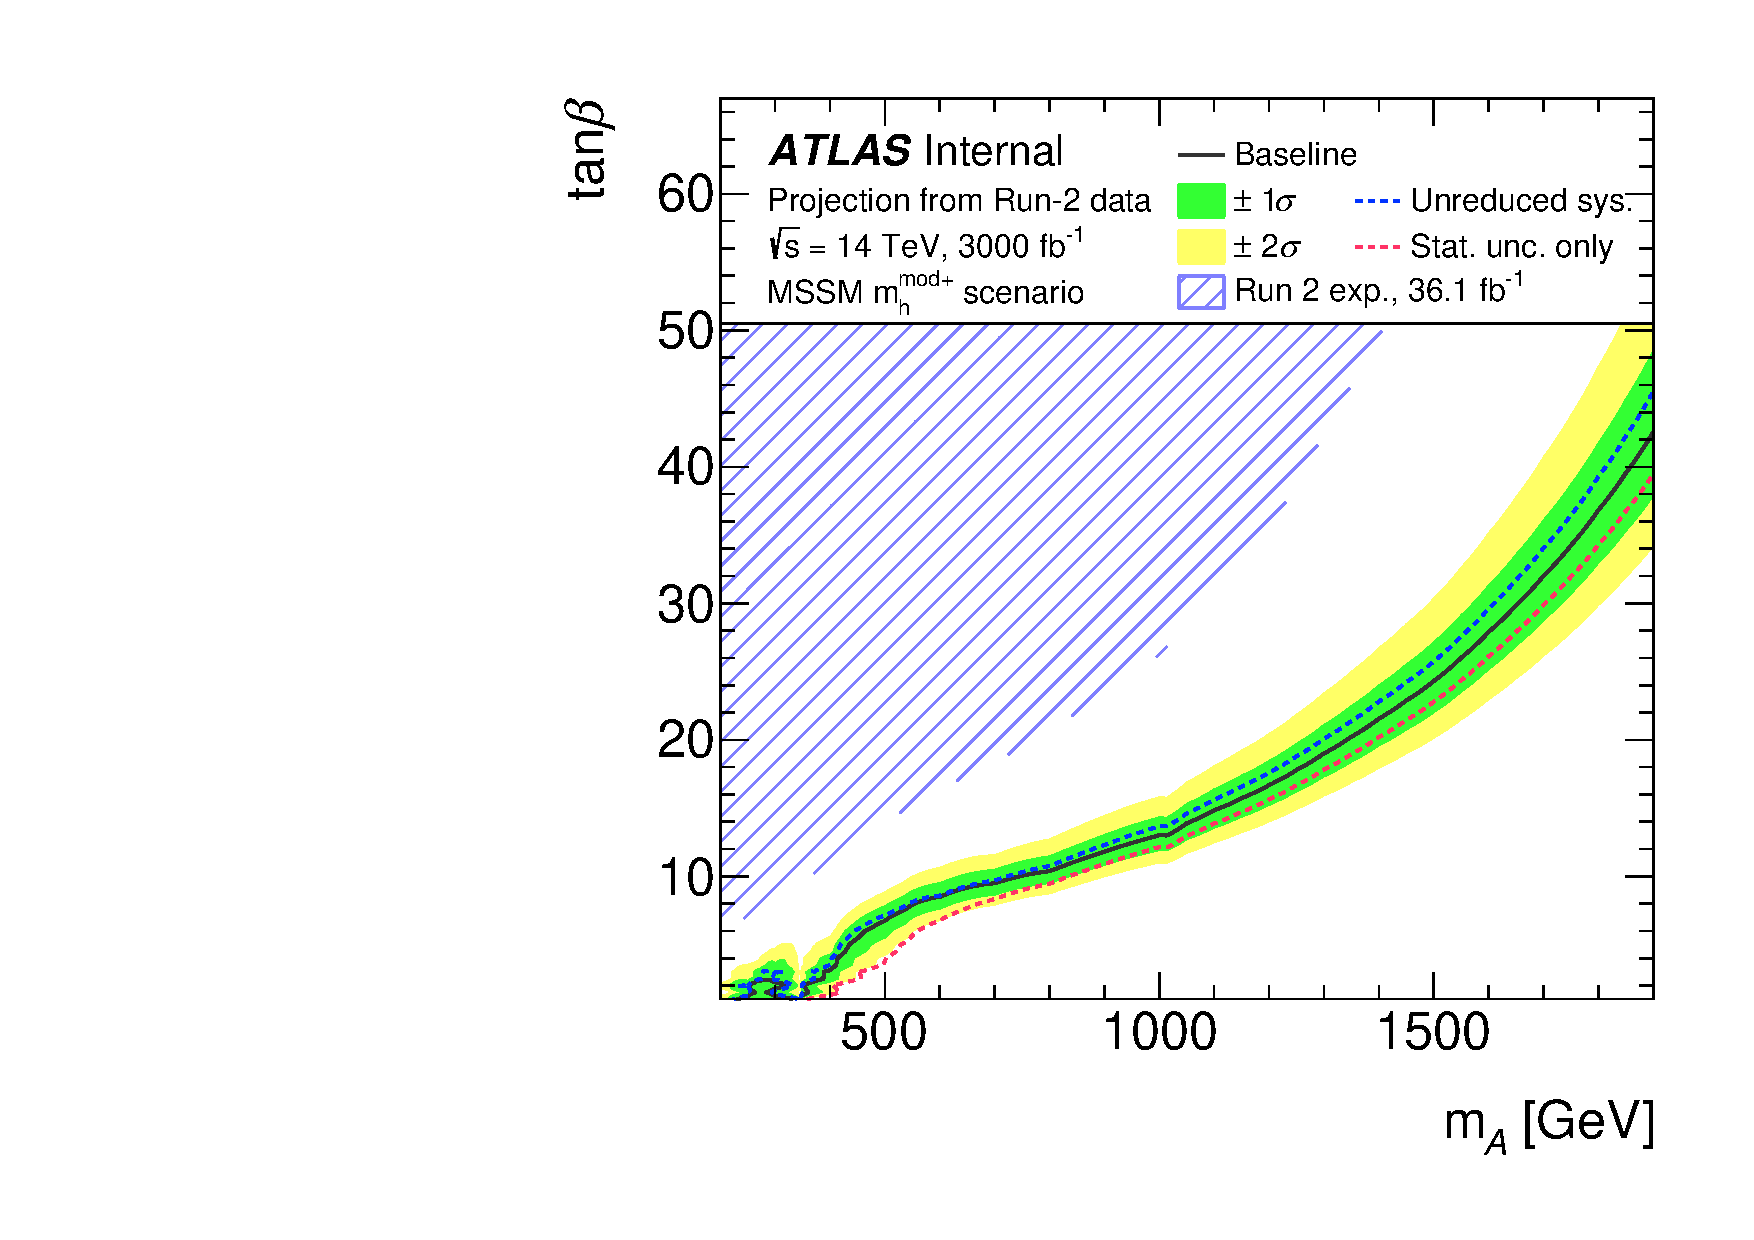
\includegraphics[width=0.4\columnwidth]{\main/section9/plots/mhmodp.pdf}}
        \caption{Projected 95\% CL limits on $\tan\beta$ as a function of $m_\phi$ in the MSSM (a) hMSSM and 
        (b) \mhmodp scenarios. ``Baseline'' uses the reduced systematic uncertainties scheme described in the text.
        ``Unreduced sys.'' uses the same systematic uncertainties as the Run 2 analysis while ignoring 
        the statistical uncertainty due to the limited data size of the signal and backgrounds. 
        ``Stat. unc. only'' represents the expected limit without considering any systematic uncertainty.}
    \label{fig:model1}
\end{figure}

\FloatBarrier

%-------------------------------------------------------------------------------
\paragraph{Conclusion}
\label{sec:conclusion}
%-------------------------------------------------------------------------------

% Place your conclusion here.
The $H/A \to \tau\tau$ analysis documented in \cite{ATLASRun2Ditau} have been extrapolated to estimate 
the sensitivity of the $\SI{3000}{\ifb}$ of the HL-LHC dataset. Upper limits on the cross section for the production of 
scalar bosons times the branching fraction to ditau final states are set at 95\% CL. A factor of 6 to 10 increase in 
the sensitivity compared to the searches with the  $\SI{36.1}{\ifb}$ Run 2 data \cite{ATLASRun2Ditau} is projected. 
The expected limits are in the range 140--0.8 fb (130--0.8 fb) for gluon-gluon fusion (b-associated) production of scalar 
bosons with masses of 0.2--2.25 TeV. In the context of the hMSSM scenario, the most stringent limits 
for the combined search exclude $\tan\beta > 1.0$ for $m_\phi < 300$ GeV and $\tan\beta >$~15 for $m_\phi = 1.5$ TeV 
at 95\% CL. The systematic uncertainties degrade the model independent exclusion limit by more than a factor of 2 
for $m_\phi<500$ GeV and about 40\% for  $m_\phi=2$ TeV. Especially, the uncertainty on high-$\pt$ $\tauhadvis$
reconstruction and identification is the dominant uncertainty at $m_\phi>1.0$ TeV. 
